\setcounter{step}{0}

\subsection{ Medové rezy }

\begin{ingredient}
  
      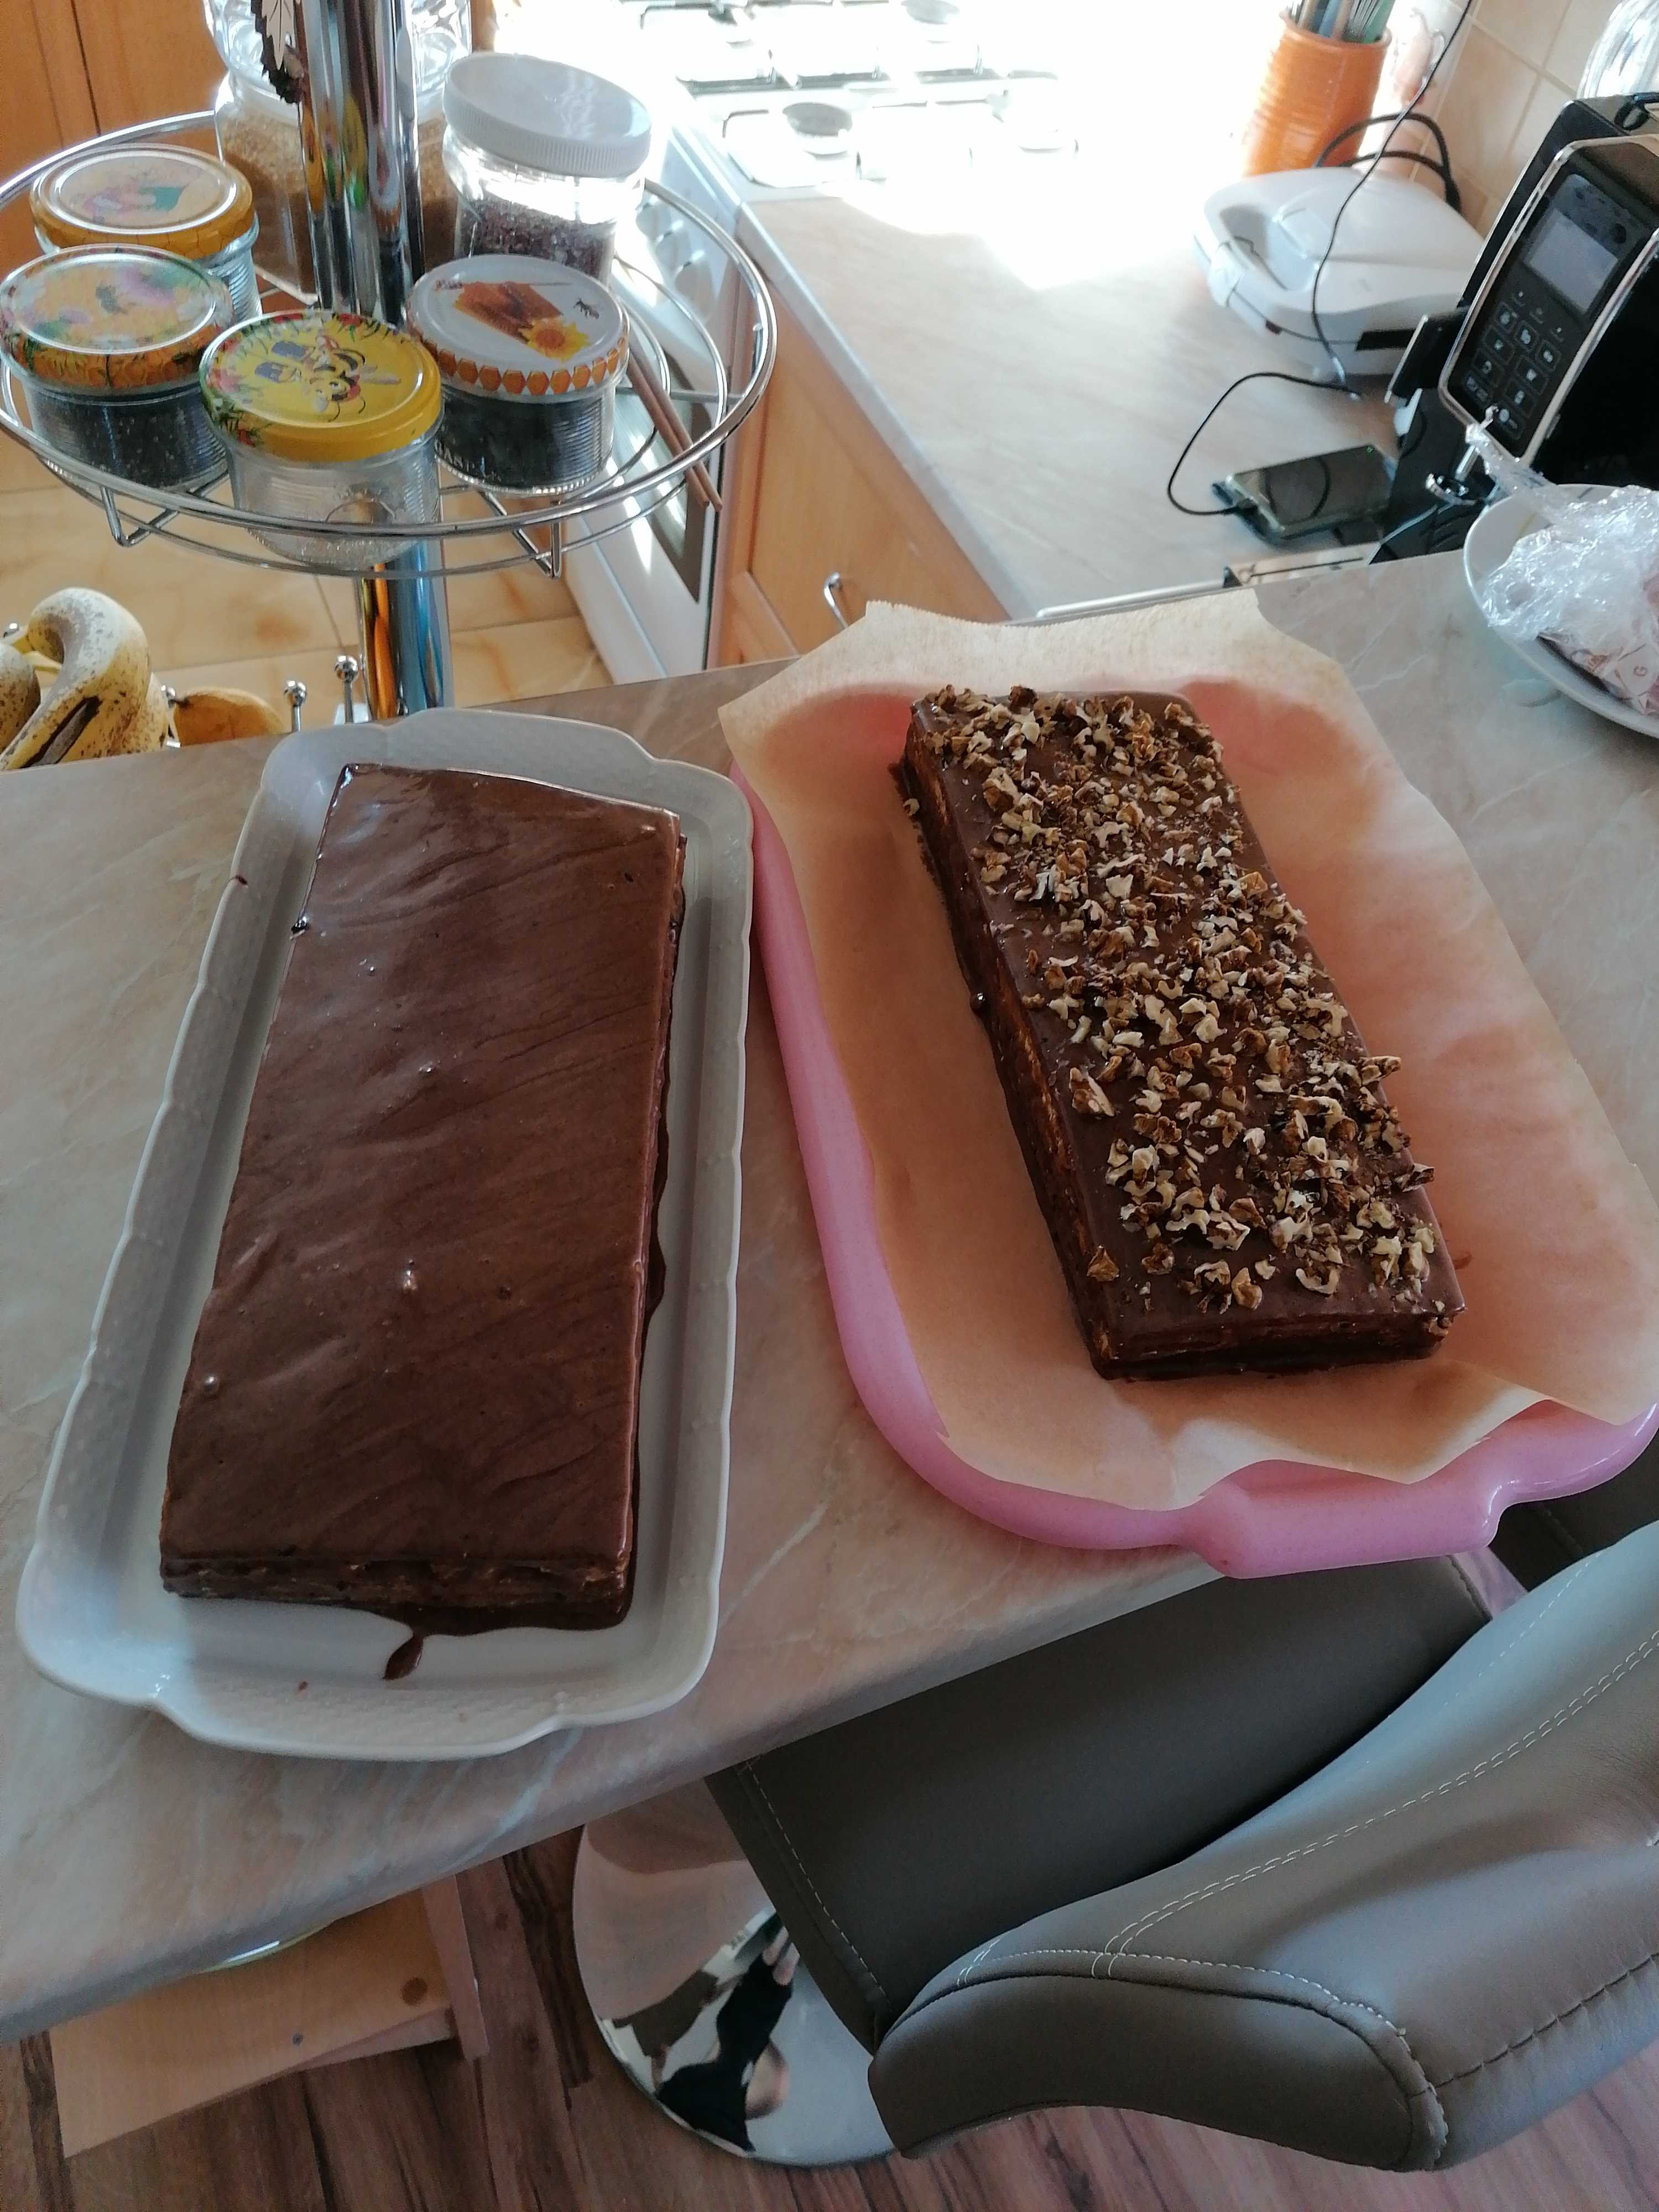
\includegraphics[height=5.5cm]{images/medove_rezy}
  
  \def\portions{  }
  \textbf{ {\normalsize Ingrediencie (20 porcie):} }

  \begin{main}
      \item 
  \end{main}
  
    \begin{subingredient}{Pláty}
        \item 2 balenia hotových plátov, alebo
        \item 250g hladká múka
        \item 250g polohrubá múka
        \item 150g cukor
        \item 80g maslo
        \item 3ks vajíčko
        \item 1 štipka sódy bikarbóny
    \end{subingredient}
  
    \begin{subingredient}{Poleva}
        \item 100g práškový cukor
        \item 100g maslo
        \item 2ks vajíčko
        \item 1PL kakao
    \end{subingredient}
  
\end{ingredient}
\begin{recipe}
\textbf{ {\normalsize Príprava:} }
\begin{enumerate}

  \item{Pripravíme pláty}
  \item{Pláty: }
      \begin{enumerate}
          \item{Nad parou zmiešame cukor, maslo, vajíčka, med, škoricu a sódu bikarbónu.}
          \item{Za stáleho miešania chvíľu varíme. Odstavíme a primiešame hladkú aj polohrubú múku.}
          \item{Z hmoty vypracujeme cesto, ktoré si rozdelíme na 4 rovnaké časti.}
          \item{Rozvaľkáme a po jednom pečieme každý plát približne 6 minút pri 180 stupňoch.}\end{enumerate}
  \item{Popri pečení pripravíme plnku: }
      \begin{enumerate}
          \item{Uvaríme Zlatý klas a necháme h vychladnúť.}
          \item{Po vychladnutí primiešame maslo a cukor.}\end{enumerate}
  \item{Na prvé dva pláty natrieme 2/3 plnky.}
  \item{Tretí potrieme džemom a na džem natrieme zvyšok plnky.}
  \item{Posledný plát položíme na tretí.}
  \item{Pripravíme polevu: }
      \begin{enumerate}
          \item{Nad parou rozšľaháme vajíčka,cukor a kakao.}
          \item{Do uvarenej horúcej zmesi vmiešame maslo.}\end{enumerate}
  \item{Naplnené pláty polejeme polevou a posypeme nasekanými orieškami.}

\end{enumerate}
\end{recipe}

\begin{notes}
  
\end{notes}	
\clearpage
